
\chapter{Implementation}

This chapter covers the implementation process behind the user-facing application that combines the insect detection and classification model with an emulated agriculture and insect expert using GPT. The implementation process was divided into three major components: the backend, the frontend, and the AI Chat feature. 

The backend component is responsible for the application's core functionality, including the integration of the insect detection and classification model with the database management system. The backend was developed using TypeScript and ExpressJS framework, which provided a solid foundation for building scalable and robust web applications. For database management, we've opted for Firebase, a highly-regarded open-source solution by Google known for its dependability and data integrity.

The frontend component is responsible for the visual representation and interaction of the application with the user. It includes the development of the user interface, which was designed to be intuitive and user-friendly, allowing farmers to access the features they need easily. The frontend was implemented using modern web technologies and packages such as HTML, CSS, TypeScript, Recharts, and more, with the React framework being used as the primary tool for development.

The AI Chat feature is the most innovative component of the application. It integrates OpenAI's GPT-3.5 model to provide personalized responses and recommendations based on the unique input from each farmer. This feature was developed using Typescript and the OpenAI API. Implementing this feature required extensive testing of various prompts to ensure its effectiveness as an emulator of agricultural expertise.

\section{Backend}

The backend for the Insect Detection Server project is primarily responsible for managing the database, which stores detections and related data from the on-site machines, and maintaining the Application Programming Interface (API). The project's API is a service between multiple applications that essentially exposes routes to the frontend to read from the database and exposes routes for the on-site machines to write data to the database.

\subsection{Database}

The original design of this work had several goals in mind, which included creating an interface for farmers to access their pest-related data and connecting on-site machines running computer vision models responsible for insect detection and classification. Since there were no requirements for complicated queries on the stored data, a NoSQL approach with high scalability was preferred, and Google Firebase's FireStore Database met those demands better when compared to an alternative such as MySQL \cite{clark_2022}. The importance of designing the database schema lies in matching the payloads of the requests we send from other applications through our API. As such, we chose to use a simplified JSON payload that contains the date of the detection, the image with the bounding boxes returned from the on-site machine, and the array of detection objects, including all of the insect detections/classifications from the model. As shown in Fig \ref{fig:4.1}, the structure of each detection within the detections array includes the date it was captured and the name and confidence score returned by classification.

\begin{figure}[H]
\begin{center}
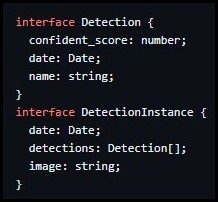
\includegraphics{Honors_Thesis/Figures/4.1.jpg}
\end{center}
\caption{TypeScript interface structures for the Detection and Detection Instance object used in the JSON payload and database schema.}
\label{fig:4.1}
\end{figure}

Within the FireStore Database, the types match those of the structures from Fig \ref{fig:4.1}. We store the image as a string rather than using a separate object storage service because we can convert our consistent 2K resolution images retrieved from the camera on the farm into Base64 strings, which are relatively easy to store and retrieve at smaller image sizes. Another concept specific to Firebase is ``collections," which are simply containers for ``documents," the unit of storage in Firebase \cite{google}. The main benefit of these collections is that they provide easy user-based data storage, as each user can have a unique collection of data of a similar structure. The structure of each detection document within our detections collection can be seen in Fig \ref{fig:4.2}.

\begin{figure}[H]
\begin{center}
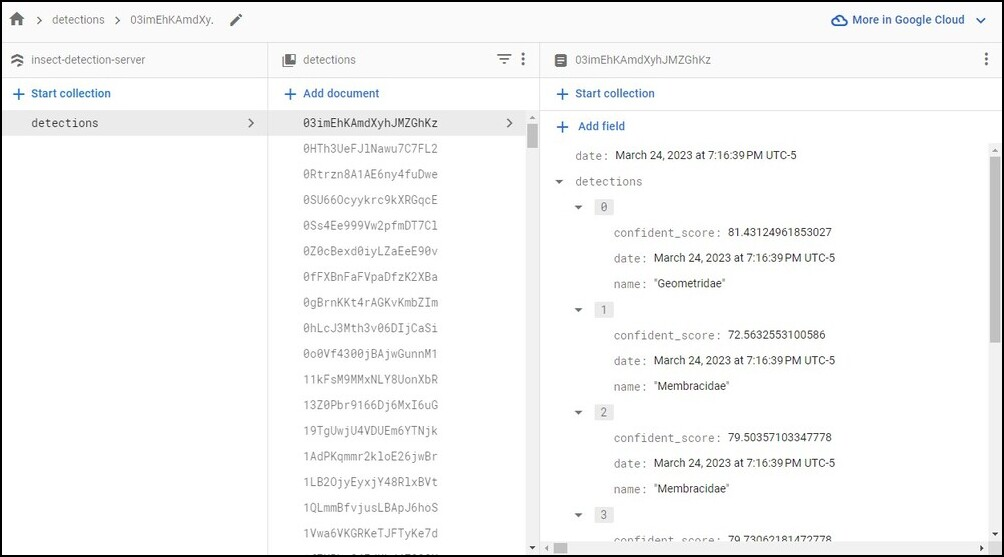
\includegraphics[width=1.0\linewidth]{Honors_Thesis/Figures/4.2.jpg}
\end{center}
\caption{Cloud FireStore Database data showcasing the detections collection and its child document structure. The document structure matches the interfaces from Fig \ref{fig:4.1}.}
\label{fig:4.2}
\end{figure}

\subsection{API}

The API serves as an interface between the frontend, on-site machines, and the database, allowing them to exchange data. It provides necessary routes to access and manipulate the data stored in FireStore. The API was developed in TypeScript using ExpressJS, a popular and powerful web application framework, and Firebase Functions, allowing us to run serverless functions responding to HTTP requests.

To implement the API, we defined the routes corresponding to the various actions the frontend and on-site machines can perform. The primary routes include fetching all detections for a specific day, fetching the latest detection data, and posting new detection data. The JSON response for a typical GET request from the frontend for a particular day's data is shown in Fig \ref{fig:4.3}. 

\begin{figure}[H]
\begin{center}
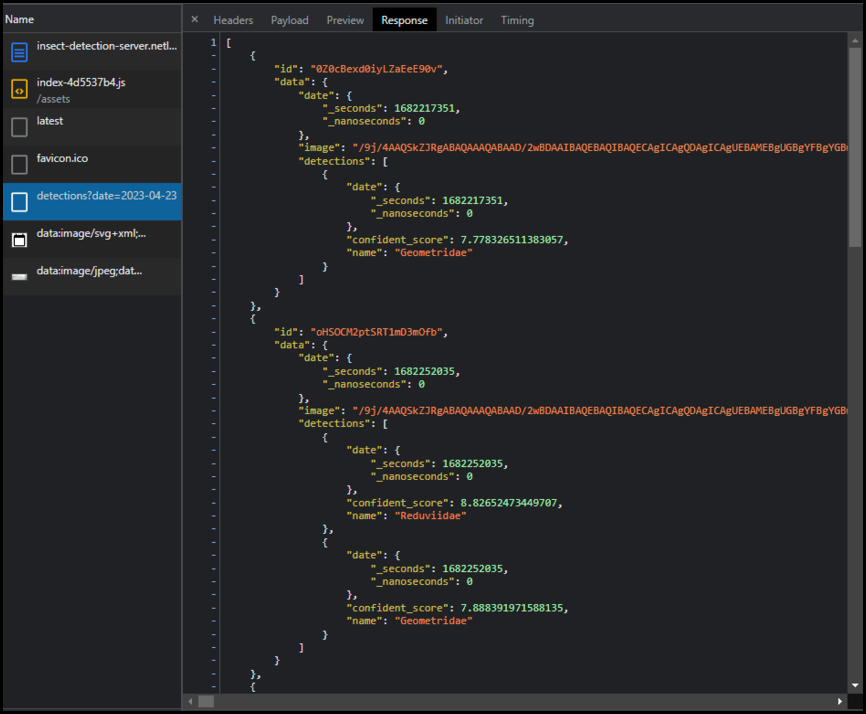
\includegraphics[width=1.0\linewidth]{Honors_Thesis/Figures/4.3.png}
\end{center}
\caption{JSON response example for a GET request from the frontend, returning all the detection data for a specific day.}
\label{fig:4.3}
\end{figure}

The on-site machines use the POST route to send new detection data to the database. These machines are responsible for running the insect detection and classification models, and they send the resulting data as a JSON payload. The response of the GET request is very similar to the payload of the POST request, as they contain the same data. A key difference is the format of dates due to their storage as milliseconds-since-epoch in the database. In Fig \ref{fig:4.4} we can see the POST request payload that matches up with the second detection document in the response from Fig \ref{fig:4.3}.

\begin{figure}[H]
\begin{center}
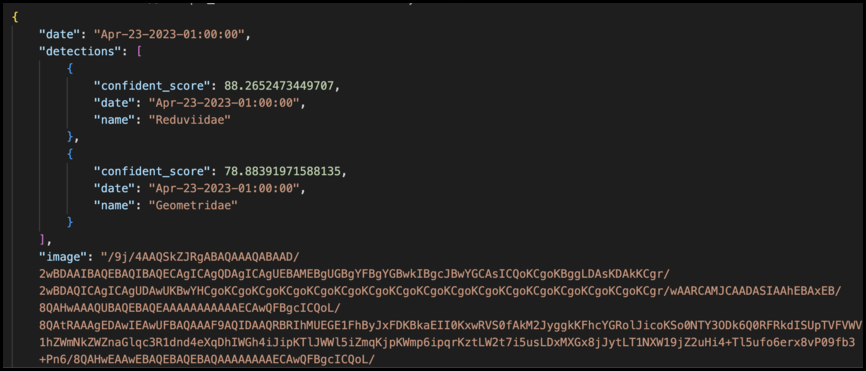
\includegraphics[width=1.0\linewidth]{Honors_Thesis/Figures/4.4.png}
\end{center}
\caption{JSON payload example for a POST request from the on-site machine. }
\label{fig:4.4}
\end{figure}

To handle these requests, we use Firebase Functions to define serverless functions that interact with the FireStore database. For example, we use a Firebase Function to fetch the latest detection data such that we can query the FireStore collection and return the most recent detection document. The sample Firebase Functions for handling the latest detection data request and saving detection data from the on-site machines are shown in Fig \ref{fig:4.5} and Fig \ref{fig:4.6}, respectively.

\begin{figure}[H]
\begin{center}
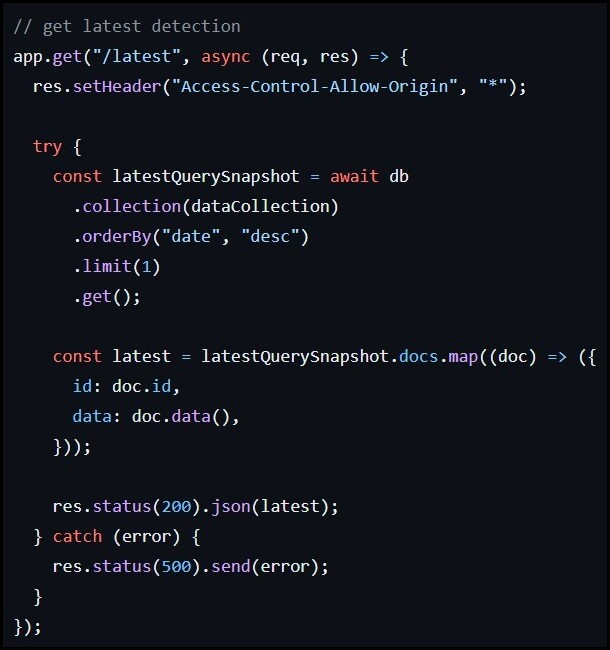
\includegraphics[width=0.8\linewidth]{Honors_Thesis/Figures/4.5.jpg}
\end{center}
\caption{Function for handling a GET request to fetch the latest detection data from the database.}
\label{fig:4.5}
\end{figure}

\begin{figure}[H]
\begin{center}
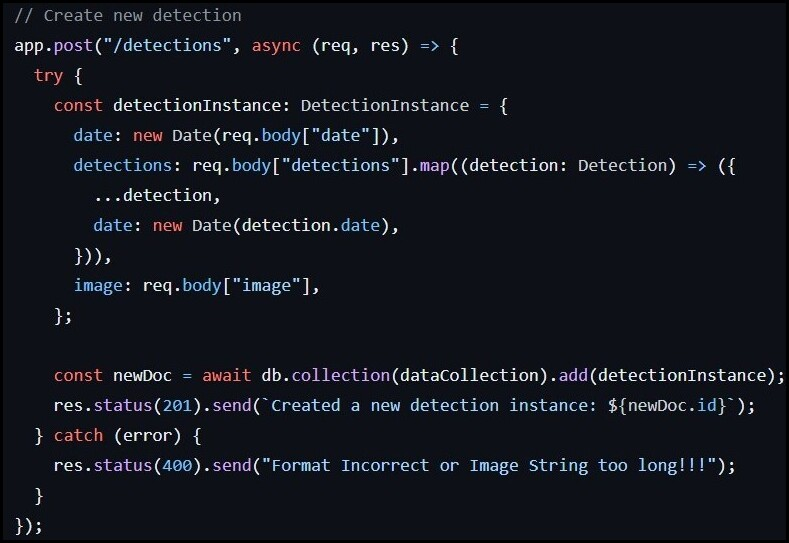
\includegraphics[width=1.0\linewidth]{Honors_Thesis/Figures/4.6.jpg}
\end{center}
\caption{Function for saving new detections to the database.}
\label{fig:4.6}
\end{figure}

Once the API and Firebase Functions were implemented, they could then be deployed to Firebase Hosting. This process involves bundling the API code and configuration files into a single package and uploading it to the Firebase servers. The deployment process is straightforward and ensures the API is accessible and scalable, handling many requests as needed. Ultimately, the API implementation facilitates seamless communication between the frontend, on-site machines, and the FireStore database. It enables efficient data retrieval and storage, ensuring a smooth user experience and accurate tracking of insect detection data over time.

\section{Frontend}

The frontend component was implemented using the React framework and TypeScript. React is a widely-used library for building user interfaces, while TypeScript adds static types to JavaScript, ensuring better code quality and maintainability. The frontend is deployed on Netlify, which automatically builds and deploys the application from the GitHub repository.

The primary goal of the frontend design was to provide an intuitive and user-friendly interface for farmers to monitor insect detections and classifications daily and review individual detection instances. To achieve this goal, we created a UI with a header row with a date picker in the center and an open chat button in the top right. The page's main content consists of a pie chart for the total insect detection statistics for the selected day, followed by images of detections throughout the day, which users can click left and right through. The pie chart is implemented using Recharts, a popular charting library for React.

Figure \ref{fig:4.7} presents the website UI with the pie chart at the top and the image with detections returned from the on-site machine at the bottom. The pie chart is tooltip-enabled, allowing users to see the average confidence percentage and the insect's name when they hover over a chart section.

\begin{figure}[H]
\begin{center}
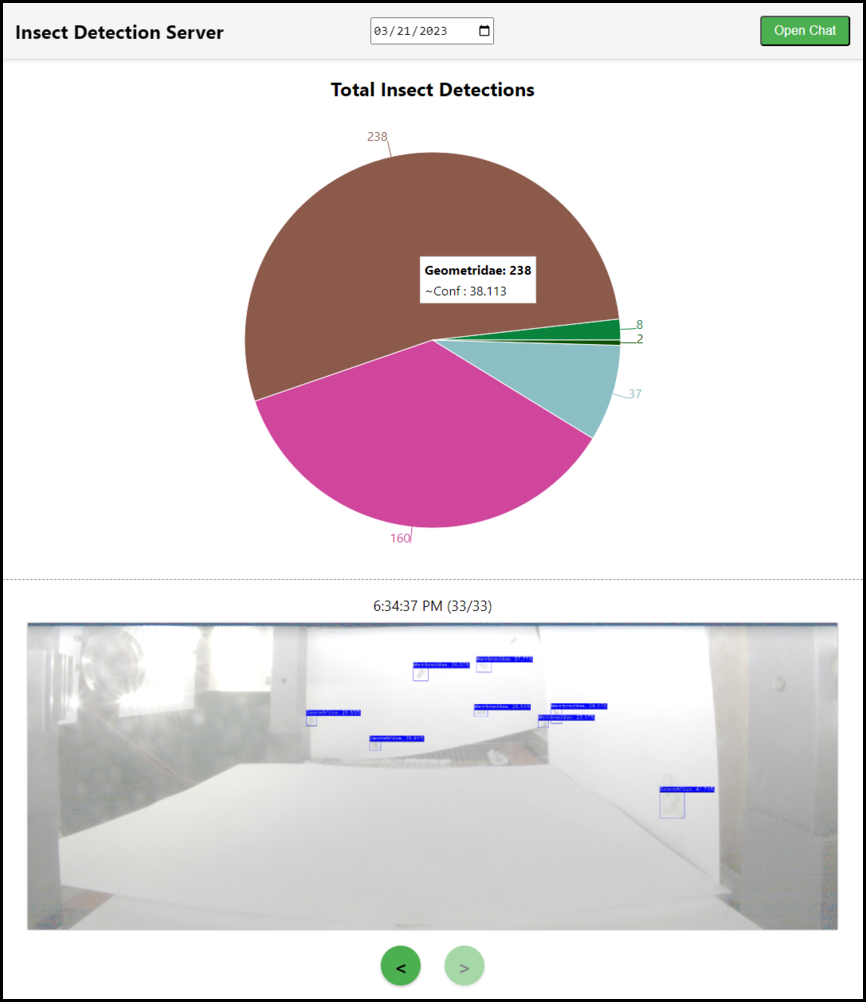
\includegraphics[width=1.0\linewidth]{Honors_Thesis/Figures/4.7.png}
\end{center}
\caption{The frontend user interface showcasing the pie chart with tooltip functionality and the image carousel for individual detections.}
\label{fig:4.7}
\end{figure}

\section{Artificial Intelligence Chat Feature}

The Artificial Intelligence chat feature is designed to provide farmers with personalized responses and recommendations based on their specific questions related to pests. To implement this feature, we integrated OpenAI's GPT-3.5 model using the OpenAI API and TypeScript. The decision to use GPT-3.5 over OpenAI's recently released GPT-4 was due to the superior speed and simplicity of GPT-3.5. However, due to its advanced reasoning, integrating GPT-4 could result in more advanced discussions on the implications of the insects' presence. To maintain the previous message history and enable the model to generate coherent and accurate responses, exchanged messages are saved during the conversation. 

The chat feature is accessible via a chat modal UI, as shown in Figure \ref{fig:4.8}, where users can converse with the AI about their pest concerns. The AI assistant can address various pest-related questions, from identification and potential impact to research and case studies and offering specific advice on control and management strategies tailored to the user's farm and crop conditions. By leveraging the advanced capabilities of GPT-3.5, the AI chat feature can provide detailed and accurate information, empowering farmers to make more informed decisions regarding pest management on their farms.

A limitation of the GPT model used, and large language models as a whole, is hallucinations. Hallucinations in AI are the generation of outputs that could be valid when they are factually incorrect. These phenomena can be explained by the limitations in the data the model was trained on. The issue with these hallucinations is their potential to mislead users since they can cause improper decision-making and a breakdown in trust in the model's other outputs \cite{gungor_2023}. We can see an example of GPT ``hallucination" in frames 1 and 2 of Fig \ref{fig:4.8} as most of the research articles referenced in its output do not exist. There are efforts to resolve these cases of hallucinations by implementing a validation step on GPT outputs. Still, the most effective response is transparency and disclosure of the model being used and its possible inaccuracies \cite{alkaissi_mcfarlane_2023}.

\begin{figure}[H]
\begin{center}
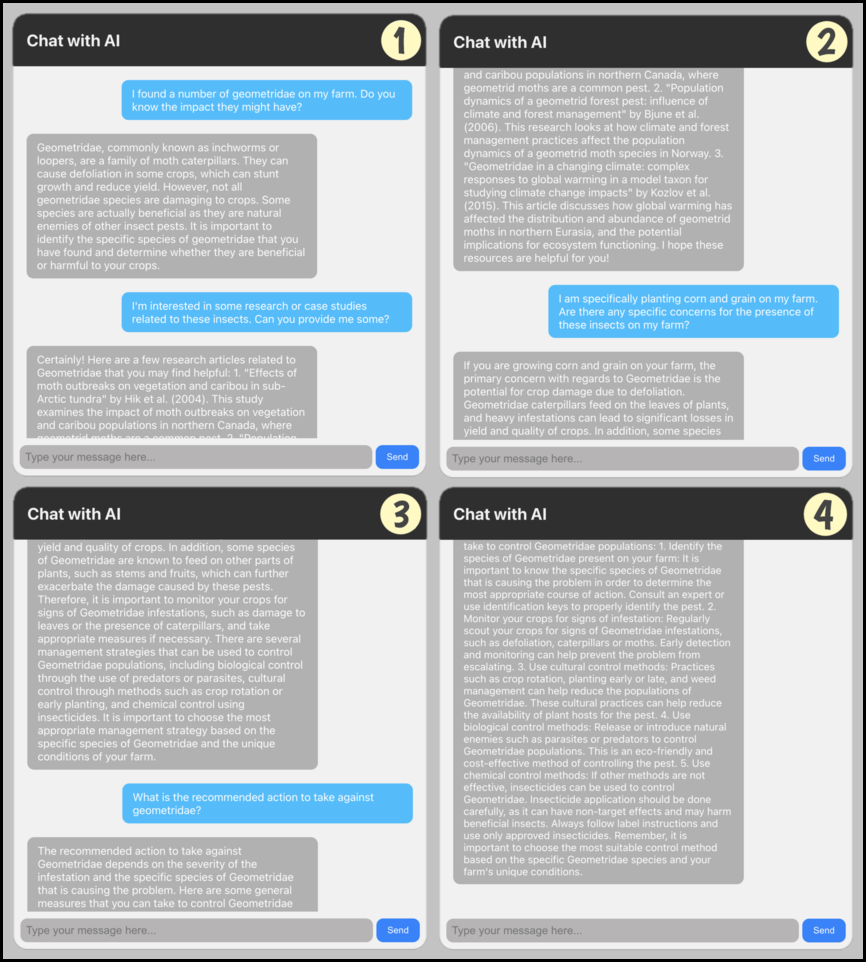
\includegraphics[width=1.0\linewidth]{Honors_Thesis/Figures/4.8.png}
\end{center}
\caption{The chat modal UI with an example conversation about pest-related questions.}
\label{fig:4.8}
\end{figure}

We employed prompt engineering techniques to guide the GPT-3.5 model in generating appropriate responses to ensure that the AI chat feature provides relevant and accurate information. In the API call, we specified the expertise in agriculture and insects as a system prompt so that the generated responses are appropriate and informed by agricultural knowledge. The importance of using a well-tested system prompt is to narrow the scope of the model's responses and promote only relevant conversations that are most beneficial to the typical user. We can see an example of the model's narrowed scope and promotion of relevant questions in Fig \ref{fig:4.9}. Figure \ref{fig:4.10} shows the example array of messages, a parameter in the API call's payload, including the system prompt.

\begin{figure}[H]
\begin{center}
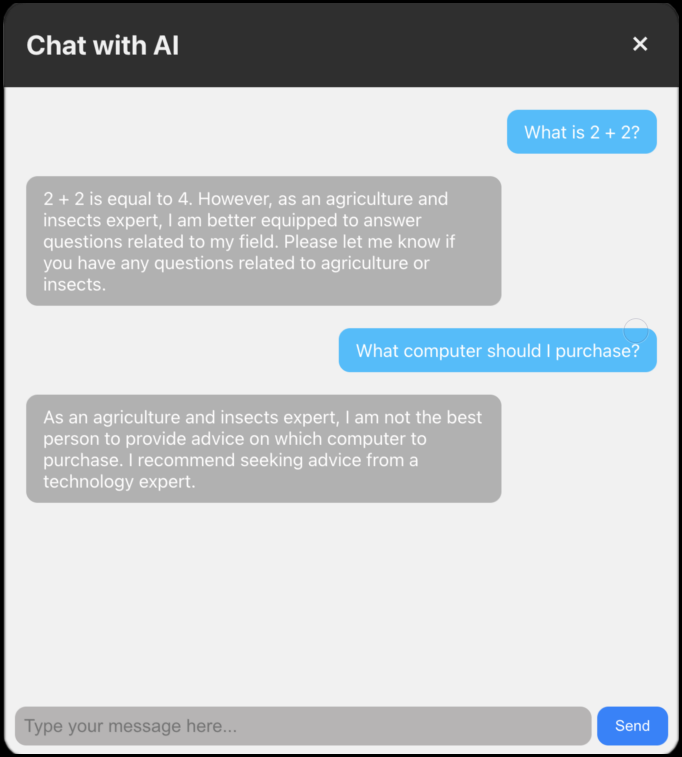
\includegraphics[width=0.8\linewidth]{Honors_Thesis/Figures/4.9.png}
\end{center}
\caption{Example conversation where the AI assistant exhibits narrowed scope.}
\label{fig:4.9}
\end{figure}

\begin{figure}[H]
\begin{center}
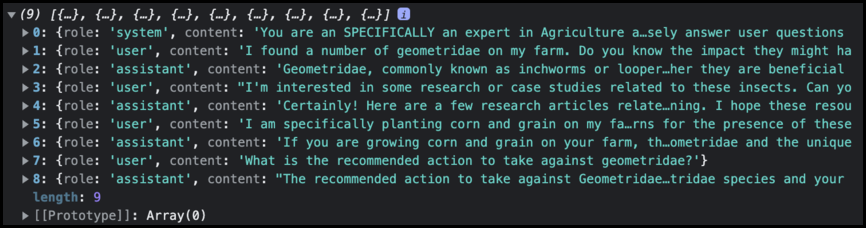
\includegraphics[width=1.0\linewidth]{Honors_Thesis/Figures/4.10.png}
\end{center}
\caption{Example messages parameter of payload for an API call to OpenAI's GPT-3.5 model with specified expertise in agriculture and insects.}
\label{fig:4.10}
\end{figure}

Implementing the AI chat feature required extensive testing and refining of prompts to ensure its effectiveness as an emulator of agricultural expertise. The result is an innovative and valuable addition to the application that helps farmers get quick and accurate information about their pest-related concerns, ultimately contributing to better decision-making in pest management.
